\subsection{Functions}

\begin{tcolorbox}[title=Problem 1, breakable]
    (a) Let $A = \{1, 2, 3\}, B = \{4\}$, and 
        $f = \{(1, 4), (2, 4), (3, 4)\}$.
        Is $f$ a function from $A$ to $B$?

    (b) Let $A = \{1\}, B = \{2, 3, 4\}$ and
        $f = \{(1, 2), (1, 3), (1, 4)\}$.
        Is $f$ a function from $A$ to $B$.

    (c) Let $C$ be the set of all cars registered
        in your state, and let $S$ be the set of all
        finite sequences of letters and digits.
        Let $L = \{(c, s) \in C \times S \mid 
            \text{the license plate number of the car $c$ is $s$}\}$.
        Is $L$ a function from $C$ to $S$.
\end{tcolorbox}

\textbf{Solution (a):}

Yes.

\textbf{Solution (b):}

No.

\textbf{Solution (c):}

Yes.

\begin{tcolorbox}[title=Problem 2, breakable]
    (a) Let $f$ be the relation represented by the graph in Figure $5.3$.
        Is $f$ a function from $A$ to $B$.

    (b) Let $W$ be the set of all words of English, and let $A$ be the set 
        of all letters of the alphabet. 
        Let 
        \[f = \{(w, a) \in W \times A \mid \text{the letter $a$ occurs in the word $w$}\}\]
        and let 
        \[g = \{(w, a) \in W \times A \mid \text{the letter $a$ is the first letter of the word $w$}\}\]
        Is $f$ a function from $W$ to $A$?
        How about $g$?

    (c) John, Mary, Susan, and Fred go out to dinner and sit at a round table.
        Let 
        \[P = \{\text{John, Mary, Susan, Fred}\}\]
        and let 
        \[R = \{(p, q) \in P \times P \mid \text{the person $p$ is sitting immediately to the right of person $q$}\}\]
        Is $R$ a function from $P$ to $P$.
\end{tcolorbox}

\begin{figure}[h]
    \centering
    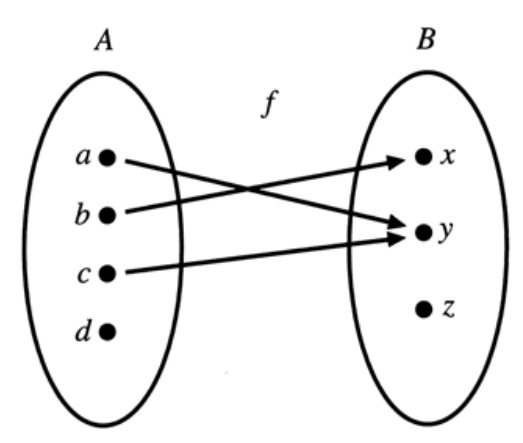
\includegraphics[width=0.4\textwidth]{images/func.png}
\end{figure}

\textbf{Solution (a):}

No.

\textbf{Solution (b):}

$f$: No.
$g$: Yes.

\textbf{Solution (c):}

Yes.

\begin{tcolorbox}[title=Problem 7, breakable]
    Suppose $f : A \rightarrow B$ and $C \subseteq A$.
    The set $f \cap (C \times B)$, which is a relation from $C$ to $B$,
        is called the \emph{restriction} of $f$ to $C$, and is sometimes
        denoted $f | C$. 
    In other words.\
    \[f | C = f \cap (C \times B)\]
    (a) Prove that $f | C$ is a function from $C$ to $B$ and that for all $c \in C$,
        $f(c) = (f | C)(c)$.

    (b) Suppose $g : C \rightarrow B$. Prove that $g = f | C$ iff $g \subseteq f$.

    (c) Let $g$ and $h$ be the functions defined in parts $2$ and $3$ of Example $5.1.3$.
        Show that $g = h | \mathbb{Z}$.
        \[g : \mathbb{Z} \rightarrow \mathbb{R} \text{ and } g(x) = 2x + 3\]
        \[h : \mathbb{R} \rightarrow \mathbb{R} \text{ and } h(x) = 2x + 3\]
\end{tcolorbox}

\begin{proof}
    We must show that $f|C$ is a function.  
    For all $x \in C$, there exists $y$ such that $(x, y) \in f|C$,  
    and there is exactly one $y \in B$ such that $(x, y) \in f|C$.

    Let $x$ be an arbitrary element in $C$.
    Since $C \subseteq A$, it follows that $x \in A$.
    Since $f$ is a function from $A$ to $B$, 
        there exists $y \in B$ such that $(x, y) \in f$.
    Clearly, $(x, y) \in A \times B$.
    Since $(x, y) \in f$ and $(x, y) \in C \times B$,
        it follows that $(x, y) \in f \cap (C \times B) = f|C$.
    Thus $f|C$ maps all elements in $C$ to $B$.

    Notice that $f \cap (C \times B) \subseteq f$.
    Then, since $(x, y) \in f|C$, it follows that $(x, y) \in f$.
    It follows that, since $f$ is a function, 
        $x$ maps to exactly one element in $B$, namely $y$.
\end{proof}

\begin{proof}
    Suppose $g : C \rightarrow B$.

    ($\rightarrow$) Suppose $g = f|C$.
    Then $g = f|C = f \cap (C \times B) \subseteq f$.

    ($\leftarrow$) Suppose $g \subseteq f$.
    Let $(x, y)$ be an arbitrary element in $g$.
    Since $g \subseteq f$, it follows that $(x, y) \in f$.
    Since $(x, y) \in g$, it follows that $(x, y) \in C \times B$.
    Thus $(x, y) \in f$ and $(x, y) \in C \times B$.
    Therefore $(x, y) \in f \cap (C \times B) = f|C$.
    It follows that $g \subseteq f|C$.

    Let $(x, y)$ be an arbitrary element in $f|C$.
    It follows that $(x, y) \in f$ and $(x, y) \in C \times B$.
    Since $g \subseteq f$ and $x \in C$, it follows that $(x, y) \in g$.
    Thus $f|C \subseteq g$.
\end{proof}

\begin{proof}
    We need to show that $g = h|\mathbb{Z} = h \cap (\mathbb{Z} \times \mathbb{R})$.
    
    Suppose $(x, y)$ is an arbitrary element in $g$.
    We know that $(x, y) \in \mathbb{Z} \times \mathbb{R}$.
    It follows that $x \in \mathbb{Z}$ and $y \in \mathbb{R}$.
    Since $\mathbb{Z} \subseteq \mathbb{R}$, it follows that $x \in \mathbb{R}$.
    Therefore $(x, y) \in h$.
    Since $(x, y) \in h$ and $(x, y) \in \mathbb{Z} \times \mathbb{R}$,
        it follows that $(x, y) \in h|\mathbb{Z}$.
    Thus $g \subseteq h|\mathbb{Z}$.

    Suppose $(x, y)$ is an arbitrary element in $h|\mathbb{Z}$.
    It follows that $(x, y) \in h$ and $(x, y) \in \mathbb{Z} \times \mathbb{R}$.
    Since $x \in \mathbb{Z}$, it follows that $(x, y) \in g$.
    Thus $h|\mathbb{Z} \subseteq g$.
\end{proof}

\begin{tcolorbox}[title=Problem 8, breakable]
    Suppose $f : A \rightarrow B$ and $g \subseteq f$.
    Prove that there is a set $A' \subseteq A$ such that 
        $g : A' \rightarrow B$.
\end{tcolorbox}

\begin{proof}
    Let $A' = dom(g)$.
    It is clear that $A' \subseteq A$,
        since $dom(g) \subseteq dom(f)$.
    Let $x \in A'$. Then there exists $y$ such that $(x, y) \in g$.
    Since $g \subseteq f$, it follows that $(x, y) \in f$.
    There is only a single element that $x$ maps to,
        since $g \subseteq f$ and $f$ is a function.
    Thus $g : A' \rightarrow B$.
\end{proof}

\begin{tcolorbox}[title=Problem 9, breakable]
    Suppose $f : A \rightarrow B$, $B \ne \emptyset$, and $A \subseteq A'$.
    Prove that there is a function $g : A' \rightarrow B$ such that $f \subseteq g$.
\end{tcolorbox}

\begin{proof}
    Let $A'' = A' \setminus A$.
    Since $B \ne \emptyset$, let $y$ be an element in $B$.
    Let $g = f \cup \{(x, y) \mid x \in A''\}$.
    Then for each $x \in A$ there is a unique $y$ such that $(x, y) \in f$,
    and for each $x \in A''$ there is exactly one pair $(x, y)$ in $g$.
    Thus $g$ is a function from $A'$ to $B$ and $f \subseteq g$.
\end{proof}

\begin{tcolorbox}[title=Problem 11, breakable]\
    Suppose $A$ is a set. 
    Show that $i_A$ is the only relation on $A$ that 
        is both an equivalence relation and also a function from $A$ to $A$.
\end{tcolorbox}

\begin{proof}
    For contradiction, suppose $R \ne i_A$ is an equivalence relation on $A$
        and $R : A \rightarrow A$.
    Then there exists a pair $(x, y) \in R$ such that $x \ne y$.
    Since $R$ is reflexive, $(x, x) \in R$.
    Thus $R$ contains both $(x, x)$ and $(x, y)$ with $y \ne x$,
        contradicting that $R$ is a function.
    Therefore $R = i_A$.
\end{proof}

\begin{tcolorbox}[title=Problem 12, breakable]
    Suppose $f : A \rightarrow C$ and $g : B \rightarrow C$.

    (a) Prove that if $A$ and $B$ are disjoint, then $f \cup g : A \cup B \rightarrow C$.

    (b) Prove that $f \cup g : A \cup B \rightarrow C$ iff $f | (A \cap B) = g | (A \cap B)$.
        (See excersize $7$ for the meaning of the notation used here.)
\end{tcolorbox}

\begin{proof}
    Suppose $A$ and $B$ are disjoint.
    Let $x$ be an arbitrary element in $A \cup B$.
    Either $x \in A$ or $x \in B$.
    If $x \in A$, then under $f$ there exists a unique $y \in C$
        such that $(x, y) \in f$.
    If $x \in B$, then under $g$ there exists a unique $y \in C$
        such that $(x, y) \in g$.
    Since $A$ and $B$ are disjoint, $f \cup g$ assigns exactly one $y \in C$
        to each $x \in A \cup B$.
    Therefore $f \cup g : A \cup B \rightarrow C$.
\end{proof}

\begin{proof}
    ($\rightarrow$) Suppose $f \cup g : A \cup B \rightarrow C$.
    For contradiction assume $f | (A \cap B) \ne g | (A \cap B)$.
    Suppose w.l.o.g. since $f | (A \cap B) \ne g | (A \cap B)$
        there is a pair $(x, y) \in f | (A \cap B)$
        such that $(x, y) \notin g | (A \cap B)$.
    Now clearly $(x, y) \in f$, but since $g$ is a function on $B$
        and $x \in A \cap B$, there is a pair $(x, y') \in g$.
    Thus $f \cup g$ results in two mappings from $x$ to $y$ and $y'$,
    which contradicts that $f \cup g$ is a function.
    Therefore, $f | (A \cap B) = g | (A \cap B)$.

    ($\leftarrow$) Suppose $f | (A \cap B) = g | (A \cap B)$.
    We must show that $f \cup g : A \cup B \rightarrow C$.
    Let $(x, y)$ and $(x, y')$ be elements of $f \cup g$.
    We need to show $y = y'$.
    If both pairs are in $f$ or both in $g$, this follows since
    $f$ and $g$ are functions.
    If one pair is from $f$ and the other from $g$, then
    $x \in A \cap B$ and hence $(x, y) \in f | (A \cap B)$
    and $(x, y') \in g | (A \cap B)$.
    By assumption $f | (A \cap B) = g | (A \cap B)$, so $y = y'$.
    Thus $f \cup g$ is a function from $A \cup B$ to $C$.
\end{proof}

\begin{tcolorbox}[title=Problem 13, breakable]
    Suppose $R$ is a relation from $A$ to $B$, $S$ is a relation 
    from $B$ to $C$, $Ran(R) = Dom(S) = B$, and $S \circ R : A \rightarrow C$.

    (a) Prove that $S : B \rightarrow C$.

    (b) Give an example to show that it need not be the case 
        that $R : A \rightarrow B$.
\end{tcolorbox}

\begin{proof}
    Let $b$ be an arbitrary element in $B$.
    Since $Ran(R) = Dom(S) = B$, there exists $a \in A$ such that $(a, b) \in R$.
    Because $S \circ R$ is a function, there is exactly one $c \in C$
        such that $(a, c) \in S \circ R$.
    By the definition of composition, this means $(a, b) \in R$ and $(b, c) \in S$.
    Thus $S$ maps $b$ to a unique $c \in C$.
    Therefore, $S : B \rightarrow C$.
\end{proof}

\textbf{Solution (b):}
\[R = \{(1, 2), (1, 3)\}, S = \{(2, 4), (3, 4)\}, S \circ R = \{(1, 4)\}\]

\begin{tcolorbox}[title=Problem 17, breakable]
    Suppose $A$ is a nonempty set and $f : A \rightarrow A$.

    (a) Suppose there is some $a \in A$ such that 
        $\forall{x} \in A(f(x) = a)$. (In this case, $f$ is called 
        a constant function.) Prove that for all $g : A \rightarrow A$,
        $f \circ g  = f$.

    (b) Suppose that for all $g : A \rightarrow A$, $f \circ g = f$.
        Prove that $f$ is a constant function. (Hint: what happens
        if $g$ is a constant function?)
\end{tcolorbox}

\begin{proof}
    Let $(x, z)$ be an arbitrary pair in $f \circ g$.
    There exists $y$ such that $(x, y) \in g$ and $(y, z) \in f$.
    It follows, since $f$ is a constant function, that $(x, z) \in f$.
    Thus $f \circ g \subseteq f$.

    Let $(x, z)$ be an arbitrary pair in $f$.
    Now, since $g : A \rightarrow A$ is a function, for this $x \in A$
        there exists a unique $y \in A$ such that $(x, y) \in g$.
    Since $f$ is a constant function and $y \in A$,
        it follows that $(y, z) \in f$.
    Since $(x, y) \in g$ and $(y, z) \in f$, 
        it follows that $(x, z) \in f \circ g$.
    Thus $f \subseteq f \circ g$.

    Therefore $f \circ g = f$.
\end{proof}

\begin{proof}
    Let $x_0 \in A$ and define 
        $g : A \to A$ such that $g(x) = x_0$ for all $x \in A$.
    Then for every $x \in A$, $(f \circ g)(x) = f(g(x)) = f(x_0)$.
    By assumption, $f \circ g = f$, so for every $x \in A$, $f(x) = (f \circ g)(x) = f(x_0)$.
    Therefore, $f$ maps every element of $A$ to the same value.
    It follows that $f$ is a constant function.
\end{proof}

\begin{tcolorbox}[title=Problem 19, breakable]
    Let $\mathcal{F} = \{f \mid f : \mathbb{Z}^+ \rightarrow \mathbb{R}\}$.
    For $g \in \mathcal{F}$, we define the set $O(g)$ as follows:
    \[O(g) = \{f \in \mathcal{F} \mid \exists{a} \in \mathbb{Z}^+
                \exists{c} \in \mathbb{R}^+ \forall{x} > a (|f(x)| \le c|g(x)|)\}\]
    (If $f \in O(g)$, then mathematicians say ``$f$ is big-oh of $g$''.)

    (a) Let $f : \mathbb{Z}^+ \rightarrow \mathbb{R}$ and $g : \mathbb{Z}^+ \rightarrow \mathbb{R}$
        be defined by the formulas $f(x) = 7x + 3$ and $g(x) = x^2$. 
        Prove that $f \in O(g)$, but $g \notin O(f)$.

    (b) Let $S = \{(f, g) \in \mathcal{F} \times \mathcal{F} \mid f \in O(g)\}$. Prove that 
        $S$ is a preorder, but not a partial order. (See excersize $25$  of Section $4.5$
        for the definition of \emph{preorder}.)

    (c) Suppose $f_1 \in O(g)$ and $f_2 \in O(g)$, and $s$ and $t$ are real numbers.
        Define a function $f : \mathbb{Z}^+ \rightarrow \mathbb{R}$ by the formula 
        $f(x) = sf_1(x) + tf_2(x)$. Prove that $f \in O(g)$.
        (Hint: You may find the triangle inequality helpful. See excersize $13$(c)
         of Section $3.5$.)
\end{tcolorbox}

\begin{proof}
    Let $a = 500$ and $c = 1$.
    Then $|f(x)| \le c|g(x)| \iff |7x + 3| \le 1|x^2|$.
    With $x \ge a = 500$ we have $7x + 3 \le x^2$.
    At the point $x = 500$, we have $7(500) + 3 = 3503 \le 500^2 = 250000$.
    To show that $|f(x)| \le c|g(x)|$ for all $x > a$, we can look at the derivatives:
        $f'(x) = 7$ and $g'(x) = 2x$, and for $x > 500$, $g'(x) > f'(x)$, so $g(x)$ grows faster than $f(x)$.
    Thus $f \in O(g)$.
\end{proof}

\begin{proof}
    Suppose $g \in O(f)$ then it follows that 
        there exists $c \in \mathbb{R}^+$ and $a \in \mathbb{Z}^+$
        such that for all $x > a$, $|g(x)| \le c|f(x)|$.
    Now plugging in gives $|x^2| \le c|7x + 3|$.
    Since $x^2$ grows faster than $7x + 3$, for any fixed $c$
        there exists $x > a$ such that $x^2 > c(7x + 3)$,
        which is a contradiction.
    Therefore, $g \notin O(f)$.
\end{proof}

\begin{proof}
    We must show $S$ is reflexive and transitive on $\mathcal{F}$.
    Suppose $f$ is an arbitrary element in $\mathcal{F}$.
    Clearly if we let $a = 1, c = 1$ then $|f(x)| \le |f(x)|$
        thus $(f, f) \in S$.

    Suppose $(f, g), (g, t)$ are arbitrary pairs in $S$.
    Now there exists $a_1 \in \mathbb{Z}^+$ and $c_1 \in \mathbb{R}^+$
        such that for all $x > a_1$,
        $|f(x)| \le c_1 |g(x)|$.
    Similarly there exists $a_2 \in \mathbb{Z}^+$ and $c_2 \in \mathbb{R}^+$
        such that for all $x > a_2$,
        $|g(x)| \le c_2 |t(x)|$.
    Let $a = \max(a_1, a_2)$. Then for all $x > a$,
        $|f(x)| \le c_1 |g(x)| \le c_1 c_2 |t(x)|$.
    Thus $(f, t) \in S$.
\end{proof}

\begin{proof}
    Since $f_1 \in O(g)$ and $f_2 \in O(g)$ it follows 
        there exists $c_1, c_2 \in \mathbb{R}^+$ and $a_1, a_2 \in \mathbb{Z}^+$
        such that for all $x > a_1$ and $x > a_2$,
        $|f_1(x)| \le c_1 |g(x)|$ and $|f_2(x)| \le c_2 |g(x)|$.
    Then since $|f_1(x)| \le c_1 |g(x)|$ it follows that 
        $|s f_1(x)| \le |s| c_1 |g(x)|$.
    Similarly $|t f_2(x)| \le |t| c_2 |g(x)|$.
    Taking sums gives 
        $|s f_1(x)| + |t f_2(x)| \le (|s| c_1 + |t| c_2)|g(x)|$.
    By the triangle inequality 
        $|s f_1(x) + t f_2(x)| \le |s f_1(x)| + |t f_2(x)|$.
    Let $a = \max(a_1, a_2)$. Then for all $x > a$
        it follows that $|s f_1(x) + t f_2(x)| \le (|s| c_1 + |t| c_2)|g(x)|$.
    Let $c = |s| c_1 + |t| c_2$. Then $|f(x)| \le c |g(x)|$ for all $x > a$,
    and therefore $f \in O(g)$.
\end{proof}

\begin{tcolorbox}[title=Problem 21, breakable]
    Suppose $f : A \rightarrow B$ and $R$ is an equivalence relation on $A$.
    We will say that $f$ is compatible with $R$ if 
    $\forall{x} \in A \forall{y} \in A (xRy \rightarrow f(x) = f(y))$.

    (a) Suppose $f$ is compatible with $R$ prove that there is a unique function 
        $h : A / R \rightarrow B$ such that for all $x \in A, h([x]_R) = f(x)$.

    (b) Suppose $h : A / R \rightarrow B$ and for all $x \in A, h([x]_R) = f(x)$.
        Prove that $f$ is compatible with $R$.
\end{tcolorbox}

\begin{proof}
    First note that since $R$ is an equivalence relation, 
        for all $x \in A$ there exists $y$ such that $xRy$.
    This follows since $R$ is reflexive, so $xRx$.
    Define a function $h : A / R \rightarrow B$ by setting 
        $h([x]_R) = f(x)$ for each $x \in A$.

    Suppose $x, y \in A$ such that $[x]_R = [y]_R$.
    Then $xRy$ and it follows since $f$ is compatible with $R$ that $f(x) = f(y)$.

    Uniqueness of $h$ follows because such a function must satisfy 
        $h([x]_R) = f(x)$ for all $x \in A$.
\end{proof}

\begin{proof}
    Let $x, y$ be arbitrary elements in $A$
        such that $(x, y) \in R$.
    Since $(x, y) \in R$ it follows that 
        $f(x) = h([x]_R) = h([y]_R) = f(y)$.
    Thus $f(x) = f(y)$.
    Therefore $f$ is compatible with $R$.
\end{proof}

\begin{tcolorbox}[title=Problem 22, breakable]
    Let $R = \{(x, y) \in \mathbb{N} \times \mathbb{N} \mid x \equiv y \pmod{5}\}$.
    Note that by Theorem $4.5.10$ and excersize $14$ in Section $4.5$, $R$ is an 
    equivalence relation on $\mathbb{N}$.

    (a) Show that there is a unique function $h : \mathbb{N} / R \rightarrow \mathbb{N} / R$
        such that for every natural number $x, h([x]_R) = [x^2]_R$. (Hint: Use excersize $21$.)

    (b) Show that there is no function $h : \mathbb{N} / R \rightarrow \mathbb{N} / R$
        such that for every natural number $x, h([x]_r) = [2^x]_R$.
\end{tcolorbox}

\begin{proof}
    Suppose $x, y \in \mathbb{N}$ such that $[x]_R = [y]_R$.
    Then $x = 5k_1 + r$ and $y = 5k_2 + r$ for some $k_1, k_2 \in \mathbb{Z}$.
    Now $x^2 = 25k_1^2 + 10k_1 r + r^2$ and $y^2 = 25k_2^2 + 10k_2 r + r^2$.
    Taking differences gives $x^2 - y^2 = 25(k_1^2 - k_2^2) + 10r(k_1 - k_2)$.
    It follows that $x^2 - y^2$ is divisible by $5$, so $[x^2]_R = [y^2]_R$.
    From problem $21$, let $A = \mathbb{N}$ and $R' = R$,
        where $R'$ refers to $R$ from the previous problem.
    Then this follows immediately.
\end{proof}

\begin{proof}
    For contradiction, suppose there exists a function $h : \mathbb{N} / R \rightarrow \mathbb{N} / R$
    such that for every natural number $x, h([x]_R) = [2^x]_R$.
    Let $x, y \in \mathbb{N}$ such that $x \ne y$ and $y \in [x]_R$.
    It follows that $h([x]_R) = h([y]_R)$, so $[2^x]_R = [2^y]_R$.
    Now let $x = 1$ and $y = 6$. Then $y \in [x]_R$ because $6 \equiv 1 \pmod{5}$.
    But $2^1 = 2 \equiv 2 \pmod{5}$ and $2^6 = 64 \equiv 4 \pmod{5}$, 
    so $[2^1]_R \ne [2^6]_R$. This is a contradiction.
\end{proof}

\subsection{One-to-One and Onto}

\begin{tcolorbox}[title=Problem 1, breakable]
    Which of the functions in exercize $1$ of Section $5.1$
        are one-to-one? Which are onto?

    (a) Let $A = \{1, 2, 3\}, B = \{4\}$, and 
        $f = \{(1, 4), (2, 4), (3, 4)\}$.
        Is $f$ a function from $A$ to $B$?

    (b) Let $A = \{1\}, B = \{2, 3, 4\}$ and
        $f = \{(1, 2), (1, 3), (1, 4)\}$.
        Is $f$ a function from $A$ to $B$.

    (c) Let $C$ be the set of all cars registered
        in your state, and let $S$ be the set of all
        finite sequences of letters and digits.
        Let $L = \{(c, s) \in C \times S \mid 
            \text{the license plate number of the car $c$ is $s$}\}$.
        Is $L$ a function from $C$ to $S$.
\end{tcolorbox}

\textbf{Solution (a):}
\begin{center}
    One-to-one: No, Onto: Yes.
\end{center}
\textbf{Solution (b):}
\begin{center}
    Was not a function.
\end{center}
\textbf{Solution (c):}
\begin{center}
    One-to-one: Yes, Onto: No (Some license plates haven't been assigned to vehicles.)
\end{center}

\begin{tcolorbox}[title=Problem 2, breakable]
    Which of the functions in exercize $2$ of Section $5.1$
        are one-to-one? Which are onto?

    (a) Let $f$ be the relation represented by the graph in Figure $5.3$.
        Is $f$ a function from $A$ to $B$.

    (b) Let $W$ be the set of all words of English, and let $A$ be the set 
        of all letters of the alphabet. 
        Let 
        \[f = \{(w, a) \in W \times A \mid \text{the letter $a$ occurs in the word $w$}\}\]
        and let 
        \[g = \{(w, a) \in W \times A \mid \text{the letter $a$ is the first letter of the word $w$}\}\]
        Is $f$ a function from $W$ to $A$?
        How about $g$?

    (c) John, Mary, Susan, and Fred go out to dinner and sit at a round table.
        Let 
        \[P = \{\text{John, Mary, Susan, Fred}\}\]
        and let 
        \[R = \{(p, q) \in P \times P \mid \text{the person $p$ is sitting immediately to the right of person $q$}\}\]
        Is $R$ a function from $P$ to $P$.
\end{tcolorbox}

\begin{figure}[h]
    \centering
    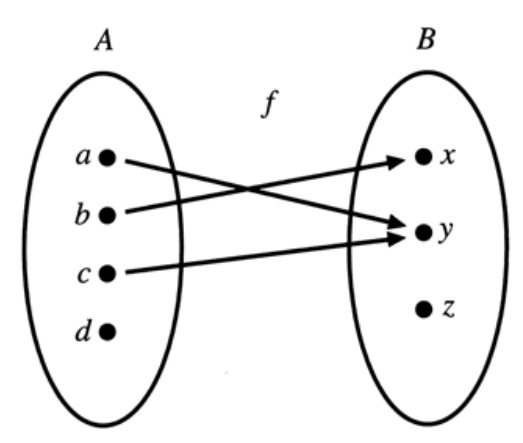
\includegraphics[width=0.4\textwidth]{images/func.png}
\end{figure}

\textbf{Solution (a):}
\begin{center}
    Was not a function.
\end{center}
\textbf{Solution (b):}
\begin{center}
    $f$ was not a function.
    $g$ One-to-one: no, Onto: yes.
\end{center}
\textbf{Solution (c):}
\begin{center}
    One-to-one: yes, Onto: yes.
\end{center}

\begin{tcolorbox}[title=Problem 3, breakable]
    Which of the functions in exercize $3$ of Section $5.1$
        are one-to-one? Which are onto?

    (a) Let $A = \{a, b, c\}, B = \{a, b\}$, and $f = \{(a, b), (b, b), (c, a)\}$.

    (b) Let $f : \mathbb{R} \rightarrow \mathbb{R}$ be the function defined by the
        formula $f(x) = x^2 - 2x$.

    (c) Let $f = \{(x, n) \in \mathbb{R} \times \mathbb{Z} \mid n \le x < n + 1\}$. 
        Then $f : \mathbb{R} \rightarrow \mathbb{Z}$.
\end{tcolorbox}

\textbf{Solution (a):}
\begin{center}
    One-to-one: no, Onto: yes.
\end{center}
\textbf{Solution (b):}
\begin{center}
    One-to-one: no, Onto: no.
\end{center}
\textbf{Solution (c):}
\begin{center}
    One-to-one: no, Onto: yes.
\end{center}

\begin{tcolorbox}[title=Problem 4, breakable]
    Which of the functions in exercize $4$ of Section $5.1$
        are one-to-one? Which are onto?

    (a) Let $N$ be the set of all countries and $C$ the set of all 
        cities. Let $H : N \rightarrow C$ be the function defined by the rule 
        that for every country $n$, $H(n) =$ the capital of the country $n$.

    (b) Let $A = \{1, 2, 3\}$ and $B = \mathcal{P}(A)$.
        Let $F : B \rightarrow B$ be the function defined by the 
            formula $F(X) = A \setminus X$.

    (c) Let $f : \mathcal{R} \rightarrow \mathcal{R}$ be the function 
        defined by the formula $f(x) = (x + 1, x - 1)$.
\end{tcolorbox}

\textbf{Solution (a):}
\begin{center}
    One-to-one: no, Onto: yes.
\end{center}
\textbf{Solution (b):}
\begin{center}
    One-to-one: yes, Onto: yes.
\end{center}
\textbf{Solution (c):}
\begin{center}
    One-to-one: yes, Onto: no.
\end{center}

\begin{tcolorbox}[title=Problem 6, breakable]
    Suppose $a$ and $b$ are real numbers and $a \ne 0$. 
    Define $f : \mathbb{R} \rightarrow \mathbb{R}$ by the 
        formula $f(x) = ax + b$.
    Show that $f$ is one-to-one and onto.
\end{tcolorbox}

\begin{proof}
    Let $x_1, x_2$ be arbitrary numbers in $\mathbb{R}$.
    Then 
    \begin{align*}
        f(x_1) &= f(x_2) \\
        \iff a(x_1) + b &= a(x_2) + b \\
        \iff a(x_1) &= a(x_2) \\
        \iff x_1 &= x_2 \quad \text{Note: $a \ne 0$}
    \end{align*}
    Thus $f$ is one-to-one.
\end{proof}

\begin{proof}
    Let $y$ be an arbitrary number in $\mathbb{R}$.
    Let $x = \frac{y - b}{a}$ which is defined since $a \ne 0$.
    Then 
    \begin{align*}
        f\left(\frac{y - b}{a}\right)
            &= a\left(\frac{y - b}{a}\right) + b \\
            &= y - b + b \\
            &= y
    \end{align*}
\end{proof}

\begin{tcolorbox}[title=Problem 8, breakable]
    Let $A = \mathcal{P}(\mathbb{R})$. 
    Define $f : \mathbb{R} \rightarrow A$
        by the formula $f(x) = \{y \in \mathbb{R} \mid y^2 < x\}$.
    
    (a) Find $f(2)$.

    (b) Is $f$ one-to-one? Is it onto?
\end{tcolorbox}

\textbf{Solution (a):}
\[f(2) = \{x \mid -\sqrt{2} < x < \sqrt{2}\}\]

\textbf{Solution (b):}
\begin{center}
    One-to-one: no, Onto: no.
\end{center}

\begin{tcolorbox}[title=Problem 10, breakable]
    Suppose $f : A \rightarrow B$ and $g : B \rightarrow C$.

    (a) Prove that if $g \circ f$ is onto then $g$ is onto.

    (b) Prove that if $g \circ f$ is one-to-one then $f$ is one-to-one.
\end{tcolorbox}

\begin{proof}
    Suppose $g \circ f$ is onto.
    Let $y$ be an arbitrary element in $C$.
    Since $g \circ f$ is onto it follows that 
        there exists $x$ such that $(g \circ f)(x) = y$.
    Then there exists $c$ such that 
        $f(x) = c$ and $g(c) = y$.
    Thus $g$ is onto.
\end{proof}

\begin{proof}
    Suppose $x_1, x_2$ are arbitrary elements in $A$
        such that $f(x_1) = f(x_2)$.
    Then applying $g$ to both sides gives 
        $(g \circ f)(x_1) = (g \circ f)(x_2)$. 
    Then since $g \circ f$ is one-to-one it follows that 
        $x_1 = x_2$.
    Thus $f$ is one-to-one.
\end{proof}

\begin{tcolorbox}[title=Problem 11, breakable]
    Suppose $f : A \rightarrow B$ and $g : B \rightarrow C$.

    (a) Prove that if $f$ is onto and $g$ is not one-to-one,
        then $g \circ f$ is not one-to-one.

    (b) Prove that if $f$ is not onto and $g$ is one-to-one, 
        then $g \circ f$ is not onto.
\end{tcolorbox}

\begin{proof}
    Suppose $f$ is onto and $g$ is not one-to-one.
    Since $g$ is not one-to-one there exist 
        $x_1, x_2 \in B$ such that $x_1 \ne x_2$ and $g(x_1) = g(x_2)$.
    Now since $f$ is onto there exist $c_1, c_2 \in A$
        such that $f(c_1) = x_1$ and $f(c_2) = x_2$.
    If $c_1 = c_2$, then $x_1 = f(c_1) = f(c_2) = x_2$, a contradiction.
    Thus $c_1 \ne c_2$.
    Then $(g \circ f)(c_1) = g(f(c_1)) = g(x_1) = g(x_2) = g(f(c_2)) = (g \circ f)(c_2)$.
    Thus $g \circ f$ is not one-to-one.
\end{proof}

\begin{proof}
    Since $f$ is not onto there exists $y \in B$
        such that for all $x \in A$, $f(x) \ne y$.
    Let $c = g(y) \in C$.
    Now if for some $x \in A$, $(g \circ f)(x) = g(y)$,
        then since $g$ is one-to-one, $f(x) = y$, a contradiction.
    Thus $g \circ f$ is not onto.
\end{proof}


\begin{tcolorbox}[title=Problem 13, breakable]
    Suppose $f : A \rightarrow B$ and $C \subseteq A$.
    In exercize $7$ of Section $5.1$ we defined 
        $f | C$ (the restriction of $f$ to $C$),
        and you showed that $f | C : C \rightarrow B$

    (a) Prove that if $f$ is one-to-one, then so is $f | C$.

    (b) Prove that if $f | C$ is onto, then so is $f$.

    (c) Give examples to show that the converses of parts (a)
        and (b) are not always true.
\end{tcolorbox}

\begin{proof}
    Suppose $f$ is one-to-one.
    Let $x_1, x_2$ be two arbitrary elements in $C$ such that $(f | C)(x_1) = (f | C)(x_2)$.
    It follows that $(x_1, (f | C)(x_1)) \in f$ and $(x_2, (f | C)(x_2)) \in f$.
    Then since $f$ is one-to-one it follows that $x_1 = x_2$.
\end{proof}

\begin{proof}
    Suppose $f | C$ is onto.
    Let $y$ be an arbitrary element in $B$.
    Since $f | C$ is onto there exists $x \in C$ such that $(f | C)(x) = y$.
    It follows that $(x, y) \in f$ thus $f(x) = y$.
    Therefore $f$ is onto.
\end{proof}

\textbf{Solution:}

Counter example: If $f | C$ is one-to-one then $f$ is one-to-one.
\[A = \{1, 2\}, B = \{1, 2\}, C = \{1\}, f = \{(1, 1), (2, 1)\}, f | C = \{(1, 1)\}\]
Counter example: If $f$ is onto then $f | C$ is onto.
\[A = \{1, 2\}, B = \{1, 2\}, C = \{1\}, f = \{(1, 1), (2, 2)\}, f | C = \{(1, 1)\}\]

\begin{tcolorbox}[title=Problem 14, breakable]
    Suppose $f : A \rightarrow B$, and there is some $b \in B$
        such that $\forall{x} \in A (f(x) = b)$.
        (Thus, $f$ is a constant function.)

    (a) Prove that if $A$ has more than one element then $f$ is 
        not one-to-one.

    (b) Prove that if $B$ has more than one element then $f$ is 
        not onto.
\end{tcolorbox}

\begin{proof}
    Suppose that $A$ has more than one element.
    Since $A$ has more than one element there exists $x_1, x_2 \in A$
        such that $x_1 \ne x_2$ and $f(x_1) = b$ and $f(x_2) = b$.
    Thus $f$ is not one-to-one.
\end{proof}

\begin{proof}
    Suppose that $B$ has more than one element.
    Then there exists $y \in B$ such that $y \ne b$.
    Since $f(x) = b$ for all $x \in A$, there does not exist $x \in A$ such that $f(x) = y$.
    Therefore, $f$ is not onto.
\end{proof}

\begin{tcolorbox}[title=Problem 15, breakable]
    Suppose $f : A \rightarrow C$, $g : B \rightarrow C$,
        and $A$ and $B$ are disjoint. In excersize 
        $12(a)$ of Section $5.1$ you proved that 
        $f \cup g : A \cup B \rightarrow C$.
    Now suppose that $f$ and $g$ are both one-to-one.
    Prove that $f \cup g$ is one-to-one iff $Ran(f)$ and $Ran(g)$
        are disjoint.
\end{tcolorbox}

\begin{proof}
    ($\rightarrow$) Suppose $f \cup g$ is one-to-one.
    For contradiction, suppose $Ran(f) \cap Ran(g) \ne \emptyset$.
    Let $y$ be an element in $Ran(f) \cap Ran(g)$.
    It follows there exists $x_1 \in A$ and $x_2 \in B$
        such that $f(x_1) = y$ and $g(x_2) = y$.
    Since $A$ and $B$ are disjoint, $x_1 \ne x_2$,
    contradicting that $f \cup g$ is one-to-one.
    Thus $Ran(f)$ and $Ran(g)$ are disjoint.

    ($\leftarrow$) Suppose $Ran(f)$ and $Ran(g)$ are disjoint.
    Suppose $x_1, x_2 \in A \cup B$ such that $(f \cup g)(x_1) = (f \cup g)(x_2)$.
    Since $A$ and $B$ are disjoint, either $x_1, x_2 \in A$ or $x_1, x_2 \in B$.
    Suppose w.l.o.g.  $x_1 \in A$ and $x_2 \in B$ but
    then $(f \cup g)(x_1) \in Ran(f)$ and $(f \cup g)(x_2) \in Ran(g)$,
        which are disjoint.
    Suppose w.l.o.g. $x_1, x_2 \in A$. Since $f$ is one-to-one, it follows that 
        $x_1 = x_2$.
    Thus $f \cup g$ is one-to-one.
\end{proof}

\begin{tcolorbox}[title=Problem 16, breakable]
    Suppose $R$ is a relation from $A$ to $B$, $S$ is a relation 
        from $B$ to $C$, $Ran(R) = Dom(S) = B$,
        and $S \circ R : A \rightarrow C$.
    In exercize $13(a)$ of Section $5.1$ you proved that 
        $S : B \rightarrow C$.
    Now prove that if $S$ is one-to-one then $R : A \rightarrow B$.
\end{tcolorbox}

\begin{proof}
    Suppose $S$ is one-to-one.
    Let $x$ be an arbitrary element in $A$.
    Since $S \circ R$ is a function, there exists $y \in C$
        such that $(S \circ R)(x) = y$.
    It follows that there exists $c \in B$ such that 
        $R(x) = c$ and $S(c) = y$.
    Thus $R$ maps each element in $A$ to some element in $B$.

    Suppose there exists $x \in A$ and $y_1, y_2 \in B$
        such that $y_1 \ne y_2$ and $(x, y_1), (x, y_2) \in R$.
    Since $Ran(R) = Dom(S)$, there exist $z_1, z_2 \in C$
        such that $(y_1, z_1) \in S$ and $(y_2, z_2) \in S$.
    Then $(x, z_1), (x, z_2) \in (S \circ R)$.
    Since $S$ is one-to-one and $y_1 \ne y_2$, it follows that $z_1 \ne z_2$,
        contradicting that $S \circ R$ is a function.
    Thus for every $x \in A$ there exists a single $y \in B$
        such that $(x, y) \in R$.
\end{proof}

\begin{tcolorbox}[title=Problem 18, breakable]
    Suppose $R$ is an equivalence relation on $A$,
        and let $g : A \rightarrow A / R$ be defined 
        by the formula $g(x) = [x]_R$, as in exersize $20(b)$
        in Section $5.1$.

    (a) Show that $g$ is onto.

    (b) Show that $g$ is one-to-one iff $R = i_A$.
\end{tcolorbox}

\begin{proof}
    Let $T$ be an arbitrary element in $A / R$.
    Since $T$ is not empty, there exists $x$ such that $T = [x]_R$.
    It follows that $g(x) = [x]_R = T$.
    Thus $g$ is onto.
\end{proof}

\begin{proof}
    ($\rightarrow$) Suppose $g$ is one-to-one.
    Let $x$ be an arbitrary element in $A$.
    Since $R$ is reflexive, $(x, x) \in R$,
        thus $x \in [x]_R$.
    Since $g$ is one-to-one, no other element in $A$
        maps to $[x]_R$.
    It follows that each equivalence class contains exactly one element,
        so $R = i_A$.

    ($\leftarrow$) Suppose $R = i_A$.
    Let $x_1, x_2$ be arbitrary elements in $A$ such that $g(x_1) = g(x_2)$.
    Then $[x_1]_R = [x_2]_R$.
    Since each equivalence class contains exactly one element, it follows that $x_1 = x_2$.
    Therefore, $g$ is one-to-one.
\end{proof}

\begin{tcolorbox}[title=Problem 19, breakable]
    Suppose $f : A \rightarrow B$, $R$ is an equivalence relation on $A$,
        and $f$ is compatible with $R$. (See exersize $21$ of Section $5.1$
        for the definition of \emph{compatible}.)
    In exercize $21(a)$ of Section $5.1$ you proved that there is a unique 
        function $h : A / R \rightarrow B$ such that for all $x \in A$,
        $h([x]_R) = f(x)$. Now prove that $h$ is one-to-one iff
        $\forall{x} \in A \forall{y} \in A (f(x) = f(y) \rightarrow xRy)$.
\end{tcolorbox}

\begin{proof}
    ($\rightarrow$) Suppose $h$ is one-to-one.
    Let $x, y$ be arbitrary elements in $A$.
    Furthermore, suppose $f(x) = f(y)$.
    It follows that $h([x]_R) = h([y]_R)$.
    Then, since $h$ is one-to-one, $[x]_R = [y]_R$.
    It follows that $(x, y) \in R$.

    ($\leftarrow$) Suppose $\forall x, y \in A, (f(x) = f(y) \rightarrow xRy)$.
    Let $x_1, x_2$ be arbitrary elements in $A$
        such that $h([x_1]_R) = h([x_2]_R)$.
    Thus $f(x_1) = f(x_2)$, and it follows that $(x_1, x_2) \in R$.
    Therefore $[x_1]_R = [x_2]_R$.
    It follows that $h$ is one-to-one.
\end{proof}

\begin{tcolorbox}[title=Problem 20, breakable]
    Suppose $A, B$, and $C$ are sets and $f : A \rightarrow B$.

    (a) Prove that if $f$ is onto, $g : B \rightarrow C$, 
        $h : B \rightarrow C$, and $g \circ f = h \circ f$,
        then $g = h$.

    (b) Suppose that $C$ has at least two elements,
        and for all functions $g$ and $h$ from $B$ to $C$,
        if $g \circ f = h \circ f$ then $g = h$.
        Prove that $f$ is onto.
\end{tcolorbox}

\begin{proof}
    Suppose $f$ is onto, $g : B \rightarrow C$, 
        $h : B \rightarrow C$, and $g \circ f = h \circ f$.
    Let $b$ be an arbitrary element in $B$.
    Since $f$ is onto, there exists $a \in A$ such that $f(a) = b$.
    Now, since $g \circ f = h \circ f$, it follows that
        $(g \circ f)(a) = (h \circ f)(a)$.
    Thus $g(f(a)) = h(f(a))$, and hence $g(b) = h(b)$.
    Since $b$ was arbitrary, $g = h$.
\end{proof}

\begin{proof}
    For contradiction, suppose $f$ is not onto.
    There exists $y \in B$ such that for all $x \in A$,
        $f(x) \ne y$.
    Let $y_1, y_2 \in C$ with $y_1 \ne y_2$.
    For all $x \in B$ let 
        $g(x) = y_1$, $h(x) = y_2$ if $x = y$; otherwise $g(x) = h(x) = y_1$.
    Clearly $g \ne h$.
    However, $g \circ f = h \circ f$ since for all $x \in A$
        $f(x) \ne y$, which is a contradiction.
    Thus $f$ is onto.
\end{proof}

\begin{tcolorbox}[title=Problem 21, breakable]
     Suppose $A, B$, and $C$ are sets and $f : B \rightarrow C$.

     (a) Prove that if $f$ is one-to-one, $g : A \rightarrow B$,
         $h : A \rightarrow B$, and $f \circ g = f \circ h$, then $g = h$.

    (b) Suppose that $A \ne \emptyset$, and for all functions $g$ and $h$
        from $A$ to $B$, if $f \circ g = f \circ h$ then $g = h$.
        Prove that $f$ is one-to-one.
\end{tcolorbox}

\begin{proof}
    Suppose $f$ is one-to-one, $g : A \rightarrow B$,
         $h : A \rightarrow B$, and $f \circ g = f \circ h$.
    Let $x$ be an arbitrary element in $A$.
    There exists $y_1, y_2$ such that $h(x) = y_1$ 
        and $g(x) = y_2$.
    Since $f \circ g = f \circ h$ it 
        follows that $f(y_1) = f(y_2)$.
    Then since $f$ is one-to-one it follows that $y_1 = y_2$.
    Therefore $g = h$. 
\end{proof}

\begin{proof}
    For contradiction, suppose $f$ is not one-to-one.
    There exist $x_1, x_2 \in B$ such that $f(x_1) = f(x_2)$
        and $x_1 \ne x_2$.
    For all $x \in A$ let $g(x) = x_1$ and $h(x) = x_2$.
    Clearly $g \ne h$.
    However, for all $x \in A$, $(f \circ g)(x) = (f \circ h)(x)$,
        which is a contradiction.
    Thus $f$ is one-to-one.
\end{proof}

\begin{tcolorbox}[title=Problem 22, breakable]
    Let $\mathcal{F} = \{f \mid f : \mathbb{R} \rightarrow \mathbb{R}\}$,
        and define a relation $R$ on $\mathcal{F}$ as follows:
    \[R = \{(f, g) \in \mathcal{F} \times \mathcal{F} \mid \exists{h} \in \mathcal{F}(f = h \circ g)\}\]

    (a) Let $f, g$, and $h$ be the functions from $\mathbb{R}$ to $\mathbb{R}$ defined by the 
        formulas $f(x) = x^2 + 1$, $g(x) = x^3 + 1$, and $h(x) = x^4 + 1$. Prove that $hRf$,
        but it is not the case $gRf$.

    (b) Prove that $R$ is a preorder. (See exercize $25$ of Section $4.5$ for the
        definition of \emph{preorder}.)

    (c) Prove that for all $f \in \mathcal{F}$, $f R i_{\mathbb{R}}$.

    (d) Prove that for all $f \in \mathcal{F}$, $i_{\mathbb{R}} R f$ iff $f$ is one-to-one.
        (Hint for right-to-left direction: Suppose $f$ is one-to-one. Let $A = Ran(f)$, and 
         let $h = f^{-1} \cup ((\mathbb{R} \setminus A) \times \{0\}))$. Now prove that 
         $h : \mathbb{R} \rightarrow \mathbb{R}$ and $i_{\mathbb{R}} = h \circ f$.

    (e) Suppose $g \in \mathcal{F}$ is a constant function; in other words, there is some 
        real number $c$ such that $\forall{x} \in \mathbb{R}(g(x) = c)$. Prove that for all 
        $f \in \mathcal{F}$, $g R f$. (Hint: See exercize $17$ of Section $5.1$.)

    (f) Suppose that $g \in \mathcal{F}$ is a constant function.
        Prove that for all $f \in \mathcal{F}$, $f R g$ iff $f$ is a constant function.

    (g) As in exercize $25$ of Section $4.5$, if we let $S = R \cap R^{-1}$, then $S$ 
        is an equivalence relation on $\mathcal{F}$. Also, there is a unique relation 
        $T$ on $\mathcal{F} / S$ such that for all $f$ and $g$ in $\mathcal{F}$,
        $[f]_S T [g]_S$ iff $f R g$, and $T$ is a partial order on $\mathcal{F} / S$.
        Prove that the set of all one-to-one functions from $\mathbb{R}$ to $\mathbb{R}$
        is the largest element of $\mathcal{F} / S$ in the partial order $T$, and the set 
        of all constant functions from $\mathbb{R}$ to $\mathbb{R}$ is the smallest element.
\end{tcolorbox}

\textbf{Solution (a):}

\begin{proof}
    Let $l(x) = x^2 - 2x + 2$. Then 
    \begin{align*}
    (l \circ f)(x) 
        &= l(f(x)) \\
        &= (x^2 + 1)^2 - 2(x^2 + 1) + 2 \\
        &= x^4 + 2x^2 + 1 - 2x^2 - 2 + 2 \\
        &= x^4 + 1 \\
        &= h
    \end{align*}
    Thus $h = l \circ f$, which shows that $(h, f) \in R$.
\end{proof}

\begin{proof}
    For contradiction, suppose $(g, f) \in R$.  
    There exists a function $h$ such that $g = h \circ f$. Then
    \[
    x^3 + 1 = h(x^2 + 1) \text{ for all } x \in \mathbb{R}.
    \]  
    Suppose $t_1, t_2 \in \mathbb{R}$ with $t_1 = -t_2 \ne 0$.  
    Then $f(t_1) = t_1^2 + 1 = f(t_2)$, but $g(t_1) \ne g(t_2)$.  
    Thus $g \ne h \circ f$ for any function $h$.
\end{proof}

\textbf{Solution (b):}

\begin{proof}
    We must show $R$ is reflexive and transitive.
    Suppose $f \in \mathcal{F}$.
    Let $h : \mathbb{R} \rightarrow \mathbb{R}$ be defined be the formula $h(y) = y$.
    Suppose $x$ is an arbitrary real number.
    Then $(h \circ f)(x) = h(f(x)) = f(x)$.
    Thus $(f, f) \in R$.
    It follows that $R$ is reflexive.
    Suppose $(f, g), (g, l)$ are arbitrary elements in $R$.
    It follows that there exists $h_1, h_2$ such that 
        $f = h_1 \circ g$ and $g = h_2 \circ l$.
    Then $f = h_1 \circ g = (h_1 \circ h_2) \circ l$.
    Thus $(f, l) \in R$.
    It follows that $R$ is transitive.
    Therefore $R$ is a  preorder.
\end{proof}

\textbf{Solution (c):}

\begin{proof}
    Let $f$ be an arbitrary element in $\mathcal{F}$.
    Furthermore, let $x$ be an arbitrary real number.
    Then $(i_{\mathbb{R}} \circ f)(x) = i_{\mathbb{R}}(f(x)) = f(x)$.
    Thus $(f, i_{\mathbb{R}}) \in R$.
\end{proof}

\textbf{Solution (d):}

\begin{proof}
    ($\rightarrow$) Let $f$ be an arbitrary element in $\mathcal{F}$.
    Suppose $(i_{\mathbb{R}}, f) \in R$.
    There exists $h$ such that $i_{\mathbb{R}} = h \circ f$.
    Let $x_1, x_2$ be arbitrary real numbers such that 
        $f(x_1) = f(x_2)$.
    Applying $h$ to both sides gives 
        $(h \circ f)(x_1) = (h \circ f)(x_2)$.
    Then $x_1 = (h \circ f)(x_1) = (h \circ f)(x_2) = x_2$.
    Thus $f$ is one-to-one.

    ($\leftarrow$) Suppose $f$ is one-to-one.
    Let $A = \mathrm{Ran}(f)$.
    Define 
    \[
        h = f^{-1} \cup ((\mathbb{R} \setminus A) \times \{0\}).
    \]
    Then for each $x \in \mathbb{R}$, either $x \in A$ or $x \in \mathbb{R} \setminus A$.
    If $x \in A$, then $h(x) = f^{-1}(x)$.
    If $x \in \mathbb{R} \setminus A$, then $h(x) = 0$.
    Thus $h$ is a function from $\mathbb{R}$ to $\mathbb{R}$.
    Furthermore, for all $x \in \mathbb{R}$,
    \[
        (h \circ f)(x) = h(f(x)) = f^{-1}(f(x)) = x.
    \]
    Thus $i_{\mathbb{R}} = h \circ f$, so $(i_{\mathbb{R}}, f) \in R$.
\end{proof}

\textbf{Solution (e):}

\begin{proof}
    Let $h$ be an arbitrary function in $\mathcal{F}$.
    By Section $5.1$ Problem $17(a)$,
        $g \circ h = g$
    Thus $(g, h) \in R$.
\end{proof}

\textbf{Solution (f):}

\begin{proof}
    Let $f$ be an arbitrary element in $\mathcal{F}$.

    ($\rightarrow$) Suppose $(f, g) \in R$.
    Then there exists $h$ such that $f = h \circ g$.
    Since $g$ is a constant function, there exists $y \in \mathbb{R}$ such that $g(x) = y$ for all $x \in \mathbb{R}$.
    Then for all $x \in \mathbb{R}$,
        $f(x) = (h \circ g)(x) = h(g(x)) = h(y)$,
    which shows that $f$ is constant.

    ($\leftarrow$) Suppose $f$ is a constant function.
    Let $c$ be a real number such that $f(x) = c$ for all $x \in \mathbb{R}$.
    Furthermore, let $h$ be a function
        from $\mathbb{R}$ to $\mathbb{R}$ such that $h(y) = c$ for all $y \in \mathbb{R}$.
    Then for all $x \in \mathbb{R}$,
        $(h \circ g)(x) = h(g(x)) = c = f(x)$.
    Thus $f = h \circ g$, so $(f, g) \in R$.
\end{proof}

\textbf{Solution (g):}

\begin{proof}
    Let $f$ be an arbitrary one-to-one function in $\mathcal{F}$.
    Let $g$ be an arbitrary function in $\mathcal{F}$.
    Since $f$ is one-to-one, $f^{-1}$ exists on $\mathrm{Ran}(f)$.
    Let $h$ be a function such that 
    \[
        h = g \circ f^{-1} \;\; \cup \;\; ((\mathbb{R} \setminus \mathrm{Ran}(f)) \times \{0\}).
    \]
    Then for all $x \in \mathbb{R}$, $(h \circ f)(x) = h(f(x)) = g(x)$.
    Thus $(g, f) \in R$.
\end{proof}


\begin{proof}
    Let $f$ be an arbitrary constant function in $\mathcal{F}$.
    Let $g$ be an arbitrary function in $\mathcal{F}$.
    From part (f) it follows that there exists $h$ 
        such that $f = h \circ g$.
    Thus $(f, g) \in R$.
\end{proof}

\begin{tcolorbox}[title=Problem 23, breakable]
    Let $f : \mathbb{N} \rightarrow \mathbb{N}$ be defined by the formula $f(n) = n$.
    Note that we could also say that $f : \mathbb{N} \rightarrow \mathbb{Z}$.
    This exersize will illustrate why,
        in Definition $5.2.1$, we defined the phrase ``$f$ maps onto $B$,''
        rather than simply ``$f$ is onto.''

    (a) Does $f$ map onto $\mathbb{N}$.

    (b) Does $f$ map onto $\mathbb{Z}$.
\end{tcolorbox}

\begin{proof}
    Yes. Let $y$ be an arbitrary natural number. Then let $x = y$.
    Clearly $f(x) = x = y$. Thus $f$ maps onto $\mathbb{N}$.
\end{proof}

\begin{proof}
    No. Suppose $f$ maps onto $\mathbb{Z}$.
    Let $y$ be an arbitrary integer such that $y < 0$.
    Since $f$ is onto, exists a natural number $x$ such that $f(x) = y$.
    Then $x = y$, but $y < 0$, contradicting
    that $x$ is a natural number. Thus $f$ does not map onto $\mathbb{Z}$.
\end{proof}

\subsection{Inverses of Functions}

\begin{tcolorbox}[title=Problem 1, breakable]
    Let $R$ be the function defined in exercise $2(c)$ of Section $5.1$.
    In exercise $2$ of Section $5.2$, you showed that $R$ is one-to-one
    and onto, so $R^{-1} : P \rightarrow P$. If $p \in P$,
        what is $R^{-1}(p)$?

    Problem $2(c)$

    John, Mary, Susan, and Fred go out to dinner and sit at a round table.
    Let 
    \[P = \{\text{John, Mary, Susan, Fred}\}\]
    and let 
    \[R = \{(p, q) \in P \times P \mid \text{the person $p$ is sitting immediately to the right of person $q$}\}\]
    Is $R$ a function from $P$ to $P$.
\end{tcolorbox}

\textbf{Solution:}
\[R^{-1}(p) = \text{The person sitting immediately to the left of person $p$}\]

\begin{tcolorbox}[title=Problem 2, breakable]
    Let $F$ be the function defined in exercise $4(b)$ of Section $5.1$.
    In exercise $4$ of Section $5.2$, you showed that $F$ is one-to-one 
    and onto, so $F^{-1} : B \rightarrow B$. If $X \in B$,
    what is $F^{-1}(X)$.

    Problem $4(b)$

    Let $A = \{1, 2, 3\}$ and $B = \mathcal{P}(A)$.
    Let $F : B \rightarrow B$ be the function defined by the 
        formula $F(X) = A \setminus X$.
\end{tcolorbox}

\textbf{Solution}
\[F^{-1}(X) = A \setminus X\]

\begin{tcolorbox}[title=Problem 3, breakable]
    Let $f : \mathbb{R} \rightarrow \mathbb{R}$ be defined by the formula 
    \[f(x) = \frac{2x + 5}{3}\]
    Show that $f$ is one-to-one and onto, and find a formula for $f^{-1}(x)$.
    (You may want to imitate the method used in the example after Theorem $5.3.2$,)
\end{tcolorbox}

\begin{proof}
    Define
    \[g(x) = \frac{3x - 5}{2}\]
    Then 
    \[(f \circ g)(x) = f(g(x)) = f(\frac{3x - 5}{2}) = \frac{2\left(\frac{3x - 5}{2}\right) + 5}{3} = \frac{3x}{3} = x\]
    Also 
    \[(g \circ f)(x) = g(f(x)) = g(\frac{2x + 5}{3}) = \frac{3\left(\frac{2x + 5}{3}\right) - 5}{2} = \frac{2x}{2} = x\]
    By Theorem $5.3.5$ it follows that $g = f^{-1}$.
    Futhermore, by Theorem $5.3.4$ it follows that $f$ is one-to-one and onto.
\end{proof}

\begin{tcolorbox}[title=Problem 8, breakable]
    (a) Prove the second half of Theorem $5.3.2$ by imitating the proof of the first half.

    (b) Give an alternative proof of the second half of Theorem $5.3.2$ by appying the 
        first half to $f^{-1}$.
\end{tcolorbox}

\begin{theorem}[$5.3.2$]
    Suppose $f$ is a function from $A$ to $B$, and suppose that $f^{-1}$
        is a function from $B$ to $A$. Then $f^{-1} \circ f = i_A$ and $f \circ f^{-1} = i_B$.
\end{theorem}

\begin{proof}
    Let $b$ be an arbitrary element in $B$.
    Let $a = f^{-1}(b) \in A$.
    Then $(b, a) \in f^{-1}$ and therefore $(a, b) \in f$
    Thus,
    \[(f \circ f^{-1})(b) = f(f^{-1}(b)) = f(a) = b = i_B(b)\]
    Since $b$ was arbitrary, it follows that $\forall{b \in B}((f \circ f^{-1})(b) = i_B(b))$,
        so $f \circ f^{-1} = i_B$. 
\end{proof}

\begin{proof}
    Let $b$ be an arbitrary element in $B$.
    Let $a = f^{-1}(b) \in A$.
    Then composing with $f^{-1} \circ f$ 
        gives 
    \[((f^{-1} \circ f) \circ f^{-1})(b) = (f^{-1} \circ f)(a)
                \implies ((f^{-1} \circ f) \circ f^{-1})(b) = a\]
    Applying $f$ gives 
    \[(f \circ (f^{-1} \circ f) \circ f^{-1})(b) = f(a)
        \implies (f \circ (f^{-1} \circ f) \circ f^{-1})(b) = b = i_B\]
    Then 
    \[(f \circ (f^{-1} \circ f) \circ f^{-1})(b) = (f \circ i_A \circ f^{-1})(b) = (f \circ f^{-1})(b)\]
    Thus $f \circ f^{-1} = i_B$.
\end{proof}

\begin{tcolorbox}[title=Problem 9, breakable]
    Prove part $2$ of Theorem $5.3.3$.
\end{tcolorbox}

\begin{theorem}[Part $2$, $5.3.3$]
    If there is a function $g : B \rightarrow A$ such that $f \circ g = i_B$
        then $f$ is onto.
\end{theorem}

\begin{proof}
    Let $b$ be an arbitrary element in $B$.
    There exists $a \in A$ such that $g(b) = a$.
    Composing with $f$ gives $(f \circ g)(b) = f(a) = i_B(b) = b$.
    Thus $f$ is onto.
\end{proof}

\begin{tcolorbox}[title=Problem 10, breakable]
    Use the following strategy to give an alternative proof  of Theorem $5.3.5$:
    
    Let $(b, a)$ be an arbitrary element of $B \times A$.
    Assume $(b, a) \in g$ and prove $(b, a) \in f^{-1}$.
    Then assume $(b, a) \in f^{-1}$ and prove $(b, a) \in g$.
\end{tcolorbox}

\begin{theorem}
    Suppose $f : A \rightarrow B$, $g : B \rightarrow A$, $g \circ f = i_A$,
        and $f \circ g = i_B$. Then $g = f^{-1}$.
\end{theorem}

\begin{proof}
    Let $(b, a)$ be an arbitrary element of $B \times A$.
    Assume $(b, a) \in g$ and therefore $g(b) = a$.
    Applying $f$ shows 
    \[(f \circ g)(b) = f(a) = i_B(b) = b\]
    Thus $(a, b) \in f$ and it follows that $(b, a) \in f^{-1}$.
    Therefore $g \subseteq f^{-1}$.
    Now, assume $(b, a) \in f^{-1}$ and therefore $(a, b) \in f$.
    It follows that $f(a) = b$.
    Applying $g$ shows 
    \[(g \circ f)(a) = g(b) = i_A(a) = a\]
    Thus $(b, a) \in g$.
    Therefore $f^{-1} \subseteq g$.
    Thus $g = f^{-1}$.
\end{proof}

\begin{tcolorbox}[title=Problem 11, breakable]
    Suppose $f : A \rightarrow B$ and $g : B \rightarrow A$.

    (a) Prove that if $f$ is one-to-one and $f \circ g = i_B$, then $g = f^{-1}$.

    (b) Prove that if $f$ is onto and $g \circ f = i_A$, then $g = f^{-1}$.

    (c) Prove that if $f \circ g = i_B$ but $g \circ f \ne i_A$, then $f$ is onto 
        but one-to-one, and $g$ is one-to-one but not onto.
\end{tcolorbox}

\begin{proof}
    Suppose $f$ is one-to-one and $f \circ g = i_B$.
    Suppose $(b, a) \in B \times A$ such that $(b, a) \in g$
        and therefore $g(b) = a$.
    Then 
    \[(f \circ g)(b) = f(a) = i_B(b) = b\]
    Thus $(a, b) \in f$ and it follows that $(b, a) \in f^{-1}$.
    Therefore $g \subseteq f^{-1}$.
    Suppose $(b, a) \in B \times A$ such that $(b, a) \in f^{-1}$.
    It follows that $(a, b) \in f$ and therefore $f(a) = b$.
    Then 
\end{proof}

\begin{tcolorbox}[title=Problem 12, breakable]
    Suppose $f : A \rightarrow B$ and $f$ is one-to-one.
    Prove that there is some set $B' \subseteq B$ 
        such that $f^{-1} : B' \rightarrow A$.
\end{tcolorbox}

\begin{proof}
    Let $B' = Ran(f) \subseteq B$.
    Since $f$ is one-to-one, for each $y \in Ran(f)$ there exists a unique $x \in A$
        such that $f(x) = y$.
    Let 
    \[
        f^{-1} : B' \rightarrow A, \quad f^{-1}(y) = x \text{ such that } f(x) = y
    \]
\end{proof}

\begin{tcolorbox}[title=Problem 13, breakable]
    Suppose $f : A \rightarrow B$ and $f$ is onto.
    Let $R = \{(x, y) \in A \times A \mid f(x) = f(y)\}$.
    By exercise $20(a)$ of Section $5.1$, $R$ is an equivalence
        relation on $A$.

    (a) Prove that there is a function $h : A / R \rightarrow B$ such that 
        for all $x \in A$, $h([x]_R) = f(x)$.
        (Hint: See exercise $21$ of Section $5.1.$)

    (b) Prove that $h$ is one-to-one and onto. (Hint: See exercise $19$ of 
        Section $5.2.$)

    (c) It follows from part (b) that $h^{-1} : B \rightarrow A / R$.
        Prove that for all $b \in B$, $h^{-1}(b) = \{x \in A \mid f(x) = b\}$.

    (d) Suppose $g : B \rightarrow A$. Prove that $f \circ g = i_B$
        iff $\forall{b} \in B(g(b) \in h^{-1}(b))$.
\end{tcolorbox}

\begin{tcolorbox}[title=Problem 14, breakable]
    Suppose $f : A \rightarrow B$, $g : B \rightarrow A$, and $f \circ g = i_B$.
    Let $A' = Ran(g) \subseteq A$.

    (a) Prove that for all $x \in A'$, $(g \circ f)(x) = x$.

    (b) Prove that $f | A'$ is a one-to-one, onto function from $A'$ to $B$
        and $g = (f | A')^{-1}$. (See exercise $7$ of Section $5.1$ for the 
        meaning of the notation here.)
\end{tcolorbox}

\begin{proof}
    Let $x$ be an arbitrary element in $Ran(g) = A' \subseteq A$.
    There exists $y$ such that $g(y) = x$.
    Then applying $g \circ $f:
    \begin{align*}
        (g \circ f \circ g)(y) &= (g \circ f)(x) \\
        \iff (g \circ i_B)(y) &= (g \circ f)(x) \\
        \iff g(y) &= (g \circ f)(x)
    \end{align*}
    Since $g(y) = x$ it follows that $(g \circ f)(x) = x$.
\end{proof}

\begin{proof}
    For all $b \in B$, $(f \circ g)(b) = i_B(b)$.
    By part (a), for all $a \in A'$, $(g \circ f)(a) = i_A(a)$.
    It follows that $g = (f | A')^{-1}$.
\end{proof}

\begin{tcolorbox}[title=Problem 15, breakable]
    Let $B = \{x \in \mathbb{R} \mid x \ge 0\}$.
    Let $f : \mathbb{R} \rightarrow B$ and $g : B \rightarrow \mathbb{R}$
    be defined by the formulas $f(x) = x^2$ and $g(x) = \sqrt{x}$.
    As we saw in part $2$ of Example $5.3.6$, $g \ne f^{-1}$.
    Show that $g = (f | B)^{-1}$.
    (Hint: See exercise $14$.)
\end{tcolorbox}

\begin{proof}
    Let $x$ be positive real number such  that $x \ge 0$.
    Note that $(f \circ g)(x) = f(\sqrt{x}) = (\sqrt{x})^2 = x$.
    Since $B = Ran(g)$ it follows immediately from exercise $14$
        that $g = (f | B)^{-1}$.
\end{proof}

\begin{tcolorbox}[title=Problem 17, breakable]
    Suppose $A$ is a set, and let $\mathcal{F} = \{f \mid f : A \rightarrow A\}$
    and $\mathcal{P} = \{f \in \mathcal{F} \mid f \text{ is one-to-one and onto}\}$.
    Define a relation $R$ on $\mathcal{F}$ as follows:
    \[R = \{(f, g) \in \mathcal{F} \times \mathcal{F} \mid \exists{h} \in \mathcal{P}(f = h^{-1} \circ g \circ h)\}\]
    (a) Prove that $R$ is an equivalence relation.

    (b) Prove that if $f R g$ then $(f \circ f) R (g \circ g)$.

    (c) For any $f \in \mathcal{F}$ and $a \in A$, if $f(a) = a$ then we say that $a$
        is a \emph{fixed point} of $f$. Prove that if $f$ has a fixed point and $f R g$,
        then $g$ also has a fixed point.
\end{tcolorbox}

\begin{proof}
    We must show $R$ is reflexive, transitive, 
        and symmetric.
    Let $f$ be an arbitrary element in $\mathcal{F}$.
    Let $h = f$ then $h^{-1} \circ f \circ h = f^{-1} \circ f \circ f = i_B \circ f = f$
    Thus $(f, f) \in R$ and therefore $R$ is reflexive.
\end{proof}

\begin{tcolorbox}[title=Problem 18, breakable]
    Suppose $f : A \rightarrow C$, $g : B \rightarrow C$, and $g$ is one-to-one and onto.
    Prove that there is a function $h : A \rightarrow B$ such that $g \circ h = f$.
\end{tcolorbox}

\begin{proof}
    Let 
    \[
        h : A \rightarrow B, \quad h(a) = b \text{ such that } g(b) = f(a).
    \]
    Such $b$ exists because $g$ is onto, and is unique because $g$ is one-to-one.
\end{proof}